\documentclass[a4paper,11pt]{article}

\usepackage[T1]{fontenc}
\usepackage[utf8]{inputenc}
\usepackage{graphicx}
\usepackage{xcolor}
\usepackage{caption}
\usepackage{listings}

\renewcommand\familydefault{\sfdefault}
\usepackage{tgheros}
\usepackage[defaultmono]{droidmono}

\usepackage{amsmath,amssymb,amsthm,textcomp}
\usepackage{enumerate}
\usepackage{multicol}
\usepackage{tikz}

\usepackage{geometry}
\usepackage{trace}
\usepackage{tcolorbox}
\tcbuselibrary{listings,skins} % For lstlisting

\geometry{total={210mm,297mm},
left=25mm,right=25mm,%
bindingoffset=0mm, top=20mm,bottom=20mm}


%\linespread{1.3}

\newcommand{\linia}{\rule{\linewidth}{0.5pt}}
\newcommand{\ano}{\text{1}}

% custom theorems if needed
\newtheoremstyle{mytheor}
    {1ex}{1ex}{\normalfont}{0pt}{\scshape}{.}{1ex}
    {{\thmname{#1 }}{\thmnumber{#2}}{\thmnote{ (#3)}}}

\theoremstyle{mytheor}
\newtheorem{defi}{Definition}

% my own titles
\makeatletter
\renewcommand{\maketitle}{
\begin{center}
\vspace{2ex}
{\huge \textsc{\@title}}
\vspace{1ex}
\\
ECN 102 - Digital Logic Design \\
Department of Electronics and Communication Engineering \\
Indian Institute of Technology, Roorkee
\linia\\
\@author \hfill \@date
\vspace{4ex}
\end{center}
}
\makeatother
%%%

% custom footers and headers
\usepackage{fancyhdr}
\pagestyle{fancy}
\lhead{}
\chead{}
\rhead{}
\lfoot{Assignment \ano - Introduction to Verilog}
\cfoot{}
\rfoot{Page \thepage}
\renewcommand{\headrulewidth}{0pt}
\renewcommand{\footrulewidth}{0pt}
%

\definecolor{vgreen}{RGB}{104,180,104}
\definecolor{vblue}{RGB}{49,49,255}
\definecolor{vorange}{RGB}{255,143,102}

\makeatletter
\newcommand*\@lbracket{[}
\newcommand*\@rbracket{]}
\newcommand*\@colon{:}
\newcommand*\colorIndex{%
    \edef\@temp{\the\lst@token}%
    \ifx\@temp\@lbracket \color{black}%
    \else\ifx\@temp\@rbracket \color{black}%
    \else\ifx\@temp\@colon \color{black}%
    \else \color{vorange}%
    \fi\fi\fi
}
\makeatother

\definecolor{codebg}{RGB}{250,250,240} 
\definecolor{greatblue}{RGB}{91,155,215} 

% Set up caption and labels for lstlistings
\DeclareCaptionFont{white}{\color{white}}
\DeclareCaptionFormat{listing}{\colorbox{greatblue}{\parbox{\textwidth}{\hspace{1cm}#1#2#3}}}
\captionsetup[lstlisting]{format=listing,labelfont=white,textfont=white}

\lstdefinestyle{verilog-style}
{
    columns=fullflexible,
    language=Verilog,
    basicstyle=\small\ttfamily,
    keywordstyle=\color{vblue},
    identifierstyle=\color{black},
    commentstyle=\color{vgreen},
    numbers=left,
    numberstyle=\color{gray},  
    numbersep=10pt,
%    tabsize=8,
    moredelim=*[s][\colorIndex]{[}{]},
    literate=*{:}{:}1,
    backgroundcolor=\color{codebg},
    framexrightmargin=0.09cm, 
    framexleftmargin=-0.09cm,
    frame=trbl,
%    framesep=10pt, 
    framerule=0pt
}

\newcommand{
  \insertverilog}[3]{
  \lstinputlisting[label=#2, caption=#3, style={verilog-style}]{#1}
}
%%%----------%%%----------%%%----------%%%----------%%%

\begin{document}

\title{Assignment \ano \\ Introduction to Verilog}

\maketitle
\section*{Hardware Description Languages}
Hardware description language (HDL) is a convienient, device independent way of representing digital logic. HDLs are helpful describing, simulating and verifying digital circuits.

\subsection*{Why not use C/C++, Java...?} 
C/C++, Java are programming languages which are very good at what they were designed for, that is programming. However describing digital circuits in programming language is difficult and often confusing, which led to development of HDLs.

\subsection*{Which HDL to use?}
Today many Hardware description languages are available, each of them are different from each other in terms of functionality, semantic and grammar. In this course however we will be using Verilog  2001.

\section*{Using Verilog 2001}
As a begininer we are going to describe and simulate simple combinational circuit with Verilog.

\section*{Design Flow}  

\begin{figure}[!t] \centering 
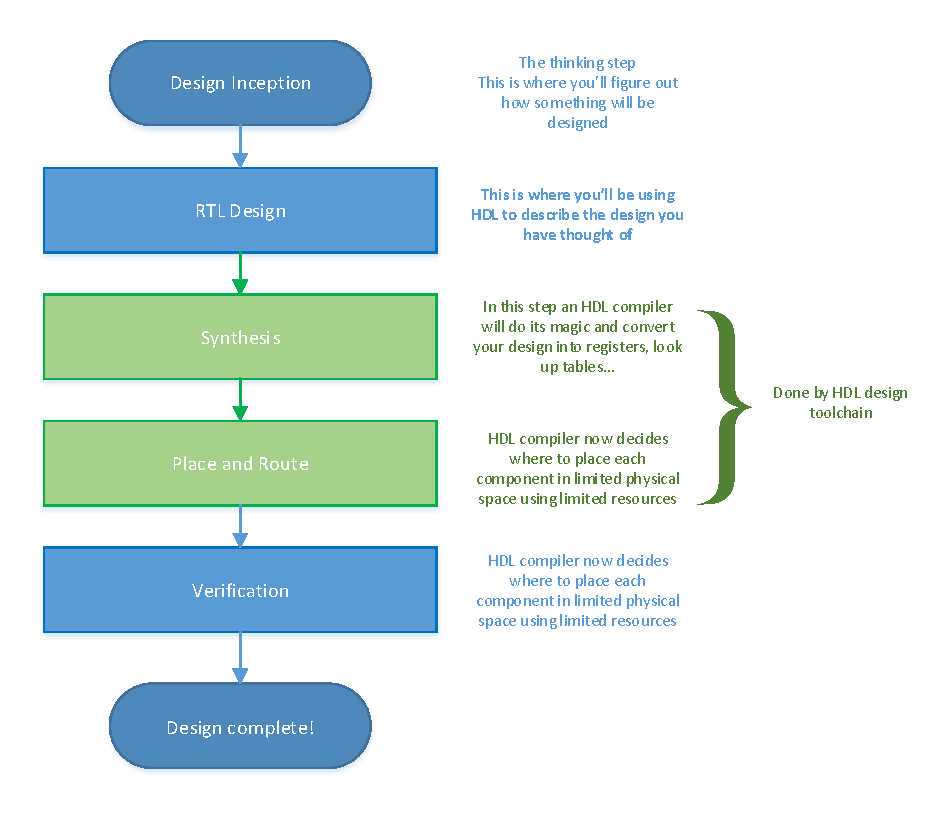
\includegraphics[width=\linewidth]{./resources/hdl_design_flow.pdf}
  \caption{Example binary search tree constructed using names from Table \ref{Table:ndn_name_table} with insertion order and output port information.}
  \label{Fig:bst_sample_names}
\end{figure} 

\section*{Verilog Syntax}
\subsection*{Modules}
Module is the basic building block in Verilog, modules helps in organizing and structuring designs in logical and human readable form. Module can be considered as analogus to functions in programming languages.

\insertverilog{./verilog_files/module.v}{sample-module}{\text{Sample module indicating its structure}}

An example of AND gate would be
\insertverilog{./verilog_files/andGate.v}{sample-module}{\text{Illustrative AND gate module}}

\subsection*{Instantiating modules}
The process of creating objects of modules is called instatiation in Verilog. Modules are a
  
\insertverilog{./verilog_files/AndGate3.v}{sample-module}{\text{Illustrative AND gate module}} 
\subsection*{Comments}
\subsection*{Numerical Literals}
\subsection*{Constants}
\subsection*{Wires}
\subsection*{Registers}
\subsection*{Always Block}
\subsection*{If and Case Statement}
% code from http://rosettacode.org/wiki/Fibonacci_sequence#Python
\begin{lstlisting}[label={list:first},caption=Sample Python code -- Fibonacci sequence calculated analytically.]
from math import *

# define function 
def analytic_fibonacci(n):
  sqrt_5 = sqrt(5);
  p = (1 + sqrt_5) / 2;
  q = 1/p;
  return int( (p**n + q**n) / sqrt_5 + 0.5 )
 
# define range
for i in range(1,31):
  print analytic_fibonacci(i)
\end{lstlisting}

Following Listing~\ref{list:first}\ldots{} 
Lorem ipsum dolor sit amet, consectetur adipiscing elit, sed do eiusmod tempor incididunt ut labore et dolore magna aliqua. Ut enim ad minim veniam, quis nostrud exercitation ullamco laboris nisi ut aliquip ex ea commodo consequat. Duis aute irure dolor in reprehenderit in voluptate velit esse cillum dolore eu fugiat nulla pariatur. Excepteur sint occaecat cupidatat non proident, sunt in culpa qui officia deserunt mollit anim id est laborum.

\section*{Problem 2}

\begin{lstlisting}[label={list:second},caption=Sample Bash code.]
#! /bin/bash
python stage1.py
echo "Stage I done!"
python stage2.py
echo "Stage II done!"
python stage3.py
echo "Stage III done!"
\end{lstlisting}

Lorem ipsum dolor sit amet, consectetur adipiscing elit, sed do eiusmod tempor incididunt ut labore et dolore magna aliqua. Ut enim ad minim veniam, quis nostrud exercitation ullamco laboris nisi ut aliquip ex ea commodo consequat. Duis aute irure dolor in reprehenderit in voluptate velit esse cillum dolore eu fugiat nulla pariatur. Excepteur sint occaecat cupidatat non proident, sunt in culpa qui officia deserunt mollit anim id est laborum.

\end{document}

%http://cva.stanford.edu/people/davidbbs/classes/ee108a/winter0607%20labs/ee108a_nham_intro_to_verilog.pdf
%Verilog HDL - Samir Palnitkar
